\documentclass[9pt,aspectratio=169]{beamer}
\usepackage{natbib}
\usepackage{bibentry}
\nobibliography*

\usepackage{color, xcolor}
\definecolor{mydarkblue}{rgb}{0,0.08,0.45}
\definecolor{mydarkred}{HTML}{990000}
\definecolor{metropolisdark}{RGB}{35,35,59}
\usepackage{overpic}
\usepackage{hyperref}
\hypersetup{
    colorlinks=true,
    citecolor=mydarkred,
    linkcolor=metropolisdark,
    urlcolor=mydarkblue
}

\usetheme[progressbar=frametitle]{metropolis}
\metroset{block=fill}
\usepackage{appendixnumberbeamer}
\usepackage{multicol}

\usepackage[absolute,overlay]{textpos}

\usepackage{nccmath}
\usepackage{caption}
\usepackage{booktabs}
\usepackage[scale=2]{ccicons}

% \usepackage{pgfplots}
% \usepgfplotslibrary{dateplot}

% Math macros to be imported into main.tex

\def\xx{{\boldsymbol x}}
\def\qq{{\boldsymbol q}}
\def\dd{{\boldsymbol d}}
\def\XX{{\boldsymbol X}}
\def\YY{{\boldsymbol Y}}
\def\ZZ{{\boldsymbol Z}}
\def\aa{{\boldsymbol a}}
\def\bb{{\boldsymbol b}}
\def\rr{{\boldsymbol r}}
\def\cc{{\boldsymbol c}}
\def\qq{{\boldsymbol q}}
\def\WW{{\boldsymbol W}}
\def\KK{{\boldsymbol K}}
\def\II{{\boldsymbol I}}
\def\yy{{\boldsymbol y}}
\def\vv{{\boldsymbol v}}
\def\uu{{\boldsymbol u}}
\def\ww{{\boldsymbol w}}
\def\zz{{\boldsymbol z}}
\def\SS{{\boldsymbol S}}
\def\BB{{\boldsymbol B}}
\def\AA{{\boldsymbol A}}
\def\CC{{\boldsymbol C}}
\def\GG{{\boldsymbol G}}
\def\FF{{\boldsymbol F}}
\def\MM{{\boldsymbol M}}
\def\DD{{\boldsymbol D}}
\def\PP{{\boldsymbol P}}
\def\TT{{\boldsymbol T}}
\def\VV{{\boldsymbol V}}
\def\OO{{\boldsymbol O}}
\def\LL{{\boldsymbol L}}
\def\HH{{\boldsymbol H}}
\def\bphi{{\boldsymbol \phi}}
\def\QQ{{\boldsymbol Q}}
\def\UU{{\boldsymbol U}}
\def\HH{{\boldsymbol H}}
\def\XX{{\boldsymbol X}}
\def\Id{{\boldsymbol{I}}}
\def\bQQ{{\textcolor{blue}{\boldsymbol Q_n}}}
\def\bbQQ{{\textcolor{blue}{\boldsymbol Q_n^{(1)}}}}
\def\rQQ{{\textcolor{red}{\boldsymbol Q}}}

\def\balpha{{\boldsymbol \alpha}}
\def\bpsi{{\boldsymbol \psi}}
\def\ttheta{{\boldsymbol \theta}}
\def\LLambda{{\boldsymbol \Lambda}}
\def\SSigma{{\boldsymbol \Sigma}}

\def\eeps{{\boldsymbol \varepsilon}}
\def\eeta{{\boldsymbol \eta}}
\def\g{{g}}
\def\ee{{\boldsymbol e}}

\def\dif{\mathop{}\!\mathrm{d}}
\def\Proba{\mathbb{P}}
\def\MP{\mu_{\mathrm{MP}}}
\def\RR{{\mathbb R}}
\def\EE{{\mathbb E}\,}
\newcommand{\Econd}{\mathbf{E}}
\renewcommand{\vec}{\mathbf{vec}}
\DeclareMathOperator{\prox}{\mathbf{prox}}
\DeclareMathOperator{\tr}{tr}
\def\defas{\stackrel{\text{def}}{=}}
\DeclareMathOperator*{\dom}{dom}
\DeclareMathOperator*{\supp}{supp}
\DeclareMathOperator*{\Fix}{Fix}
\DeclareMathOperator*{\Var}{Var}
\DeclareMathOperator*{\argmin}{{arg\,min}}
\DeclareMathOperator*{\minimize}{minimize}
\DeclareMathOperator*{\diag}{\mathbf{diag}}

\newcommand{\Prto}[1]{
  { \xrightarrow[ #1 \to \infty]{\Pr }}
}

% \DeclareDocumentCommand{\Asto} {o} {
%   \IfNoValueTF {#1}
%   {\overset{\text{\rm a.s.}}{\longrightarrow}}
%   { \xrightarrow[ #1 \to \infty]{\text{\rm a.s.} }}
% }

\newcommand{\blue}{\color{blue}}

\definecolor{myblue}{HTML}{D2E4FC}
\newcommand*\mybluebox[1]{\colorbox{myblue}{\hspace{1em}#1\hspace{1em}}}

% !TEX root = non_convex_Courtney.tex

% Macros for the Non-Convex Catalyst Paper

%% !TEX root = non_convex_Courtney.tex

% Macros for the Non-Convex Catalyst Paper

%% !TEX root = non_convex_Courtney.tex

% Macros for the Non-Convex Catalyst Paper

%\input{macros}

\newcommand{\vs}{}
%\newcommand{\vs}{\vspace*{0.0cm}}
\newcommand{\cnt}{k}
\newcommand{\pr}{{\rm prox}}
\newcommand{\eg}{\emph{e.g.}}

\renewcommand\epsilon\varepsilon
%\newcommand{\dom}{\textrm{dom }} %counter
\newcommand{\smthpara}{\kappa} % the smoothing parameter 
\newcommand{\smthparacvx}{\kappa_{\text{\rm cvx}}} % the smoothing
                                % parameter  convex
\newcommand{\smthparainit}{\kappa_0} 
\newcommand{\env}{f_{\smthpara}}
 % envelope of the prox; f_\kappa(x; y) = f(x) + kappa/2 ||x-y||^2
\newcommand{\accx}{\tilde{x}} %the \acc_x \approx argmin f_{\kappa}(x;y_k)
\newcommand{\proxx}{\bar{x}} %the \proxx \approx argmin f_{\kappa}(x;
                             %x_{k-1})
\newcommand{\bproxx}{\bar{x}^{b}} %the \proxx \approx argmin f_{\kappa}(x;
                         
                            %x_{k-1})
%\newcommand{\prox}{p_{\frac{1}{\smthpara} f}} %writes prox: kappa f ->
                                %1/kappa f
% \newcommand{\prox}{\text{prox}} 
\newcommand{\weakcnx}{\rho} %weak convexity parameter
% \newcommand{\argmin}{\operatornamewithlimits{argmin}} %argmin
\newcommand{\sccnt}{i} %Outer counter for strong convexity
\newcommand{\scnx}{\mu} %Strong convexity constant
\newcommand{\smth}{L} %smooth parameter \beta->L
\newcommand{\globalcnt}{b} %global counter for complexity
\newcommand{\li}{\operatornamewithlimits{liminf}} %argmin
%\newcommand{\mtd}{\mathcal{M}} %optimization method M used as sub-routine

%% Strong Convexity w/ Estimate Sequences %%%%%%%%%%
\newcommand{\estseqpara}{\lambda} %Estimating sequence constants
\newcommand{\estseq}{\Phi} %Estimating sequence functions
\newcommand{\estseqquad}{\gamma} %Constant multiplied by the
                                %quad. term in estimating sequence
\newcommand{\estseqcenter}{\estseq^*} % center of the estimating sequence
%% General Math %%%%%%%%%%%%%%
\newcommand{\ip}[1] {\langle #1 \rangle } %inner product
\newcommand{\norm}[1] {\left \| #1 \right \|} %norm
\newcommand{\dist}{{\rm dist}} %distance
\newcommand{\R}{{\mathbb R}} %Real numbers
\newcommand{\N}{{\mathbb N}} %Natural numbers
\newcommand{\mtd}{{\mathcal M}} %Optimization method M
\newcommand{\proxi}{\text{prox}} %proximal operator
\newcommand{\Real}{{\mathbb R}} %Real numbers
\newcommand{\oR}{\overline \R} %Reals + infinity


%%%%%%%%% Theorems %%%%%%%%%%%%%
%\newtheorem{claim}{Claim}
%\newtheorem{theorem}{Theorem}[section]
%\newtheorem{proposition}[theorem]{Proposition}
%\newtheorem{lemma}[theorem]{Lemma}
%\newtheorem{defn}[theorem]{Definition}
%\newtheorem{corollary}{Corollary}[section]
%\newtheorem{pa}{Part}
%\newtheorem{subclaim}{Subclaim}
%\newtheorem{example}{Example}[section]

%%%Random stuff%%%
\newcommand{{\newalgosp}}{Basic 4WD-Catalyst~}%basic algo, with small space after the name
\newcommand{{\newalgo}}{Basic 4WD-Catalyst}%basic algo, no space
\newcommand{{\autonewalgosp}}{4WD-Catalyst~}%adaptive algo, with small space after the name , it was before 4WD-Catalyst-Automatic
\newcommand{{\autonewalgo}}{4WD-Catalyst}%adaptive algo, no space it was before 4WD-Catalyst-Automatic
\newcommand{\linesearch}{{Auto-adapt}}

\newcommand{\mylabel}[2]{#2\def\@currentlabel{#2}\label{#1}}
\newcommand{\mynote}[1]{{\bf \color{blue}{#1} }\\}


\newcommand{\vs}{}
%\newcommand{\vs}{\vspace*{0.0cm}}
\newcommand{\cnt}{k}
\newcommand{\pr}{{\rm prox}}
\newcommand{\eg}{\emph{e.g.}}

\renewcommand\epsilon\varepsilon
%\newcommand{\dom}{\textrm{dom }} %counter
\newcommand{\smthpara}{\kappa} % the smoothing parameter 
\newcommand{\smthparacvx}{\kappa_{\text{\rm cvx}}} % the smoothing
                                % parameter  convex
\newcommand{\smthparainit}{\kappa_0} 
\newcommand{\env}{f_{\smthpara}}
 % envelope of the prox; f_\kappa(x; y) = f(x) + kappa/2 ||x-y||^2
\newcommand{\accx}{\tilde{x}} %the \acc_x \approx argmin f_{\kappa}(x;y_k)
\newcommand{\proxx}{\bar{x}} %the \proxx \approx argmin f_{\kappa}(x;
                             %x_{k-1})
\newcommand{\bproxx}{\bar{x}^{b}} %the \proxx \approx argmin f_{\kappa}(x;
                         
                            %x_{k-1})
%\newcommand{\prox}{p_{\frac{1}{\smthpara} f}} %writes prox: kappa f ->
                                %1/kappa f
% \newcommand{\prox}{\text{prox}} 
\newcommand{\weakcnx}{\rho} %weak convexity parameter
% \newcommand{\argmin}{\operatornamewithlimits{argmin}} %argmin
\newcommand{\sccnt}{i} %Outer counter for strong convexity
\newcommand{\scnx}{\mu} %Strong convexity constant
\newcommand{\smth}{L} %smooth parameter \beta->L
\newcommand{\globalcnt}{b} %global counter for complexity
\newcommand{\li}{\operatornamewithlimits{liminf}} %argmin
%\newcommand{\mtd}{\mathcal{M}} %optimization method M used as sub-routine

%% Strong Convexity w/ Estimate Sequences %%%%%%%%%%
\newcommand{\estseqpara}{\lambda} %Estimating sequence constants
\newcommand{\estseq}{\Phi} %Estimating sequence functions
\newcommand{\estseqquad}{\gamma} %Constant multiplied by the
                                %quad. term in estimating sequence
\newcommand{\estseqcenter}{\estseq^*} % center of the estimating sequence
%% General Math %%%%%%%%%%%%%%
\newcommand{\ip}[1] {\langle #1 \rangle } %inner product
\newcommand{\norm}[1] {\left \| #1 \right \|} %norm
\newcommand{\dist}{{\rm dist}} %distance
\newcommand{\R}{{\mathbb R}} %Real numbers
\newcommand{\N}{{\mathbb N}} %Natural numbers
\newcommand{\mtd}{{\mathcal M}} %Optimization method M
\newcommand{\proxi}{\text{prox}} %proximal operator
\newcommand{\Real}{{\mathbb R}} %Real numbers
\newcommand{\oR}{\overline \R} %Reals + infinity


%%%%%%%%% Theorems %%%%%%%%%%%%%
%\newtheorem{claim}{Claim}
%\newtheorem{theorem}{Theorem}[section]
%\newtheorem{proposition}[theorem]{Proposition}
%\newtheorem{lemma}[theorem]{Lemma}
%\newtheorem{defn}[theorem]{Definition}
%\newtheorem{corollary}{Corollary}[section]
%\newtheorem{pa}{Part}
%\newtheorem{subclaim}{Subclaim}
%\newtheorem{example}{Example}[section]

%%%Random stuff%%%
\newcommand{{\newalgosp}}{Basic 4WD-Catalyst~}%basic algo, with small space after the name
\newcommand{{\newalgo}}{Basic 4WD-Catalyst}%basic algo, no space
\newcommand{{\autonewalgosp}}{4WD-Catalyst~}%adaptive algo, with small space after the name , it was before 4WD-Catalyst-Automatic
\newcommand{{\autonewalgo}}{4WD-Catalyst}%adaptive algo, no space it was before 4WD-Catalyst-Automatic
\newcommand{\linesearch}{{Auto-adapt}}

\newcommand{\mylabel}[2]{#2\def\@currentlabel{#2}\label{#1}}
\newcommand{\mynote}[1]{{\bf \color{blue}{#1} }\\}


\newcommand{\vs}{}
%\newcommand{\vs}{\vspace*{0.0cm}}
\newcommand{\cnt}{k}
\newcommand{\pr}{{\rm prox}}
\newcommand{\eg}{\emph{e.g.}}

\renewcommand\epsilon\varepsilon
%\newcommand{\dom}{\textrm{dom }} %counter
\newcommand{\smthpara}{\kappa} % the smoothing parameter 
\newcommand{\smthparacvx}{\kappa_{\text{\rm cvx}}} % the smoothing
                                % parameter  convex
\newcommand{\smthparainit}{\kappa_0} 
\newcommand{\env}{f_{\smthpara}}
 % envelope of the prox; f_\kappa(x; y) = f(x) + kappa/2 ||x-y||^2
\newcommand{\accx}{\tilde{x}} %the \acc_x \approx argmin f_{\kappa}(x;y_k)
\newcommand{\proxx}{\bar{x}} %the \proxx \approx argmin f_{\kappa}(x;
                             %x_{k-1})
\newcommand{\bproxx}{\bar{x}^{b}} %the \proxx \approx argmin f_{\kappa}(x;
                         
                            %x_{k-1})
%\newcommand{\prox}{p_{\frac{1}{\smthpara} f}} %writes prox: kappa f ->
                                %1/kappa f
% \newcommand{\prox}{\text{prox}} 
\newcommand{\weakcnx}{\rho} %weak convexity parameter
% \newcommand{\argmin}{\operatornamewithlimits{argmin}} %argmin
\newcommand{\sccnt}{i} %Outer counter for strong convexity
\newcommand{\scnx}{\mu} %Strong convexity constant
\newcommand{\smth}{L} %smooth parameter \beta->L
\newcommand{\globalcnt}{b} %global counter for complexity
\newcommand{\li}{\operatornamewithlimits{liminf}} %argmin
%\newcommand{\mtd}{\mathcal{M}} %optimization method M used as sub-routine

%% Strong Convexity w/ Estimate Sequences %%%%%%%%%%
\newcommand{\estseqpara}{\lambda} %Estimating sequence constants
\newcommand{\estseq}{\Phi} %Estimating sequence functions
\newcommand{\estseqquad}{\gamma} %Constant multiplied by the
                                %quad. term in estimating sequence
\newcommand{\estseqcenter}{\estseq^*} % center of the estimating sequence
%% General Math %%%%%%%%%%%%%%
\newcommand{\ip}[1] {\langle #1 \rangle } %inner product
\newcommand{\norm}[1] {\left \| #1 \right \|} %norm
\newcommand{\dist}{{\rm dist}} %distance
\newcommand{\R}{{\mathbb R}} %Real numbers
\newcommand{\N}{{\mathbb N}} %Natural numbers
\newcommand{\mtd}{{\mathcal M}} %Optimization method M
\newcommand{\proxi}{\text{prox}} %proximal operator
\newcommand{\Real}{{\mathbb R}} %Real numbers
\newcommand{\oR}{\overline \R} %Reals + infinity


%%%%%%%%% Theorems %%%%%%%%%%%%%
%\newtheorem{claim}{Claim}
%\newtheorem{theorem}{Theorem}[section]
%\newtheorem{proposition}[theorem]{Proposition}
%\newtheorem{lemma}[theorem]{Lemma}
%\newtheorem{defn}[theorem]{Definition}
%\newtheorem{corollary}{Corollary}[section]
%\newtheorem{pa}{Part}
%\newtheorem{subclaim}{Subclaim}
%\newtheorem{example}{Example}[section]

%%%Random stuff%%%
\newcommand{{\newalgosp}}{Basic 4WD-Catalyst~}%basic algo, with small space after the name
\newcommand{{\newalgo}}{Basic 4WD-Catalyst}%basic algo, no space
\newcommand{{\autonewalgosp}}{4WD-Catalyst~}%adaptive algo, with small space after the name , it was before 4WD-Catalyst-Automatic
\newcommand{{\autonewalgo}}{4WD-Catalyst}%adaptive algo, no space it was before 4WD-Catalyst-Automatic
\newcommand{\linesearch}{{Auto-adapt}}

\newcommand{\mylabel}[2]{#2\def\@currentlabel{#2}\label{#1}}
\newcommand{\mynote}[1]{{\bf \color{blue}{#1} }\\}

\usepackage{minted}
\usepackage[version=4]{mhchem}

\usepackage{tikz}
\usetikzlibrary{shadows,calc,backgrounds,matrix,fit}



% code adapted from https://tex.stackexchange.com/a/11483/3954

% some parameters for customization
\def\shadowshift{3pt,-3pt}
\def\shadowradius{6pt}

\colorlet{innercolor}{black!60}
\colorlet{outercolor}{gray!05}

% this draws a shadow under a rectangle node
\newcommand\drawshadow[1]{
    \begin{pgfonlayer}{shadow}
        \shade[outercolor,inner color=innercolor,outer color=outercolor] ($(#1.south west)+(\shadowshift)+(\shadowradius/2,\shadowradius/2)$) circle (\shadowradius);
        \shade[outercolor,inner color=innercolor,outer color=outercolor] ($(#1.north west)+(\shadowshift)+(\shadowradius/2,-\shadowradius/2)$) circle (\shadowradius);
        \shade[outercolor,inner color=innercolor,outer color=outercolor] ($(#1.south east)+(\shadowshift)+(-\shadowradius/2,\shadowradius/2)$) circle (\shadowradius);
        \shade[outercolor,inner color=innercolor,outer color=outercolor] ($(#1.north east)+(\shadowshift)+(-\shadowradius/2,-\shadowradius/2)$) circle (\shadowradius);
        \shade[top color=innercolor,bottom color=outercolor] ($(#1.south west)+(\shadowshift)+(\shadowradius/2,-\shadowradius/2)$) rectangle ($(#1.south east)+(\shadowshift)+(-\shadowradius/2,\shadowradius/2)$);
        \shade[left color=innercolor,right color=outercolor] ($(#1.south east)+(\shadowshift)+(-\shadowradius/2,\shadowradius/2)$) rectangle ($(#1.north east)+(\shadowshift)+(\shadowradius/2,-\shadowradius/2)$);
        \shade[bottom color=innercolor,top color=outercolor] ($(#1.north west)+(\shadowshift)+(\shadowradius/2,-\shadowradius/2)$) rectangle ($(#1.north east)+(\shadowshift)+(-\shadowradius/2,\shadowradius/2)$);
        \shade[outercolor,right color=innercolor,left color=outercolor] ($(#1.south west)+(\shadowshift)+(-\shadowradius/2,\shadowradius/2)$) rectangle ($(#1.north west)+(\shadowshift)+(\shadowradius/2,-\shadowradius/2)$);
        \filldraw ($(#1.south west)+(\shadowshift)+(\shadowradius/2,\shadowradius/2)$) rectangle ($(#1.north east)+(\shadowshift)-(\shadowradius/2,\shadowradius/2)$);
    \end{pgfonlayer}
}

% create a shadow layer, so that we don't need to worry about overdrawing other things
\pgfdeclarelayer{shadow} 
\pgfsetlayers{shadow,main}

\newsavebox\mybox
\newlength\mylen

\newcommand\shadowimage[2][]{%
\setbox0=\hbox{\includegraphics[#1]{#2}}
\setlength\mylen{\wd0}
\ifnum\mylen<\ht0
\setlength\mylen{\ht0}
\fi
\divide \mylen by 120
\def\shadowshift{\mylen,-\mylen}
\def\shadowradius{\the\dimexpr\mylen+\mylen+\mylen\relax}
\begin{tikzpicture}
\node[anchor=south west,inner sep=0] (image) at (0,0) {\includegraphics[#1]{#2}};
\drawshadow{image}
\end{tikzpicture}}

\usepackage{xspace}
\newcommand{\themename}{\textbf{\textsc{metropolis}}\xspace}

\definecolor{myorange}{RGB}{217,95,2}

\newcommand{\To}[1]{
  { \xrightarrow[ ]{#1 \to \infty }}
}

\title{Random Matrix Theory for Machine Learning}
\subtitle{{\bfseries Part 3}: Analysis of numerical algorithms}
% \date{\today}
\date{}
\author{Fabian Pedregosa$^1$, Courtney Paquette$^{1, 2}$, \underline{Tom Trogdon}$^3$, Jeffrey Pennington$^1$}
\institute{
$^1$ Google Research\,, $^2$ McGill University\,, $^3$ University of Washington\\
\\
\url{https://random-matrix-learning.github.io}
}



\begin{document}

\maketitle

\begin{frame}{Notation}
In this section:
\begin{itemize}
    \item $\AA$ is typically a rectangular matrix with more rows than columns
    \item $\WW$ is a symmetric (square) matrix
    \item Often $\WW \propto \AA^T \AA$
\end{itemize}
    
\end{frame}

\section{Motivation:  Average-case versus worst-case in high dimensions}

\begin{frame}{Issues with worst-case bounds in high dimensions}

In some very specific cases, the high-dimensionality of a given problem provides it with enough degrees of freedom to ``conspire against" a given algorithm.

\pause

For, example, consider solving a $n \times n$ linear system $\WW \xx = \bb$ using the conjugate gradient (CG) algorithm  where 
\begin{align*}
    \WW = \begin{bmatrix} \mathfrak{r} & \sqrt{\mathfrak{r}} \\
    \sqrt{\mathfrak{r}} & 1 + \mathfrak{r} & \sqrt{\mathfrak{r}}\\
    & \sqrt{\mathfrak{r}} & 1 + \mathfrak{r} & \sqrt{\mathfrak{r}} \\
    && \sqrt{\mathfrak{r}}  & \ddots & \ddots \\
    &&& \ddots\\
    &&&&& \sqrt{\mathfrak{r}}\\
    &&&& \sqrt{\mathfrak{r}} & 1 + \mathfrak{r}\end{bmatrix}, \quad \bb = \begin{bmatrix} 1 \\ 0 \\ \vdots \\ 0 \end{bmatrix}, \quad 0 < \mathfrak{r} < 1.
\end{align*}
\end{frame}

\begin{frame}{Issues with worst-case bounds in high dimensions}
  The CG algorithm is iterative and produces approximations $\xx_k$ that satisfy:
  \begin{align*}
      \xx_k  = \underset{\yy \in \mathbb R^n}{\mathrm{arg}\,\mathrm{min}} \left\{  (\xx - \yy)^T \WW (\xx - \yy)^T : \yy \in \mathrm{span} \{ \bb, \WW\bb, \ldots, \WW^{k-1} \bb  \right\}.
  \end{align*}
  \pause
  
  It can be shown that for the above choice of $\WW, \bb$, and $1 \leq k < n$
  \begin{align*}
      \|\bb - \WW \xx_k\|^2 = \left( \frac{1}{\mathfrak{r}} \right)^k \quad \text{but} \quad \|\bb - \WW \xx_n\| = 0.
  \end{align*}
    \pause
    The residuals (or norms of the gradient) appear to diverge exponentially before the iteration finally converges!
    
    
    \pause
    And as $n$ increases, this becomes worse.  And a worst-case bound needs to account for this pathological example.
\end{frame}


\begin{frame}{Introducing distributions}

Instead, we may want to choose $\WW$ and $\bb$ to be random and consider
\begin{align*}
      \mathbb E\|\bb - \WW \xx_k\|^2.
\end{align*}
If one chooses $\WW$ to be distributed according to the Wishart distribution, as $n \to \infty$,
\begin{align*}
      \mathbb E\|\bb - \WW \xx_k\|^2 = \mathfrak{r}^k + o(1), \quad \mathfrak r = r^{-1} = \lim_{n\to \infty} \frac{n}{d}.
\end{align*}
\pause

But a valid important open problem is: To model optimization in a ML context, what distribution is relevant for $\WW$? 


This is an open problem.  See \cite{Liao2021} for work in this direction.


\end{frame}

\section{Main RMT tool:  Matrix moments}

\begin{frame}{Main linear algebra tool}
Recall Cauchy's integral formula:  If $f$ is analytic in a sufficiently large region and $\mathcal C$ is smooth, simple, closed curve then
\begin{align*}
    f(z) = \frac{1}{2 \pi \mathrm i} \int_{\mathcal C} \frac{f(z')}{z' - z} \dif z'.
\end{align*}
\pause

Suppose the eigenvalues of an $n \times n$ matrix $\WW$ are enclosed by $\mathcal C$, then
\begin{align*}
    f(\WW) := \UU f(\boldsymbol \Lambda) \UU^{-1} = \frac{1}{2 \pi \mathrm i} \int_{\mathcal C} f(z)( z \II_n - \WW)^{-1} \dif z.
\end{align*}

\pause

In particular,
\begin{align*}
    \WW^k = \frac{1}{2 \pi \mathrm i} \int_{\mathcal C} z^k(z \II_n - \WW)^{-1} \dif z.
\end{align*}

\end{frame}

\begin{frame}{Two consequences}

\begin{align*}
    \frac{1}{n}\mathrm{tr}\,\WW^k = \only<1>{ \frac{1}{2 \pi n \mathrm i} \int_{\mathcal C} z^k  \mathrm{tr}\, (z\II_n - W)^{-1} \dif z}\only<2->{\frac{1}{n} \sum_{j=1}^n \frac{1}{2 \pi \mathrm i} \int_{\mathcal C} z^k(z - \lambda_j)^{-1} \dif z}   \uncover<3->{= \frac{1}{2 \pi \mathrm i} \int_{\mathcal C} z^k \underbrace{m_{\mathrm{ESD}}(z)}_{\substack{\text{Stieltjes transform of} \\ n^{-1} \sum_j \delta_{\lambda_j} }} \dif z}
\end{align*}

\pause
\pause
\pause

\begin{align*}
    \uu^T\,\WW^k \uu = \uncover<5->{ \frac{1}{2 \pi \mathrm i} \int_{\mathcal C} z^k\uu^T(z \II_n - \WW)^{-1}\uu \dif z}  \uncover<6->{ = \frac{1}{2 \pi \mathrm i} \int_{\mathcal C} z^k \underbrace{m_{\mathrm{ESD}}(z)}_{\substack{\text{Stieltjes transform of} \\  \sum_j w_j \delta_{\lambda_j} }} \dif z}
\end{align*}

\pause \pause

\begin{align*}
    \sum_j w_j \delta_{\lambda_j}, \quad  w_j = (\vv_j^T \uu)^2
\end{align*}

\end{frame}


\begin{frame}{Analysis of matrix moments}
%TODO: Add CIF.  Motivate random data by worst-case can be very far from what is typical in high dimensions.

    A main RMT takeaway:
    \only<1>{\begin{center}
        Matrix moments \textcolor{red}{$\Leftrightarrow$} Classical moments of ESD  \textcolor{red}{$\Leftrightarrow$} Contour integrals of Stieltjes transform
    \end{center}}
    \only<2-5>{\begin{center}
        $\frac{1}{n}\mathrm{tr}\, \WW^k$ \only<1-2,4->{\textcolor{red}{$\approx$}}\only<3>{\textcolor{blue}{$=$}} $\displaystyle \int_{\mathbb R} x^k \mu_{\mathrm{ESD}}(\dif x)$ \only<1-3,6->{\textcolor{red}{$\approx$}}\only<4-5>{\textcolor{blue}{$=$}} $\displaystyle \frac{1}{2 \pi \mathrm{i}}\int_{\mathcal C} z^k m_{\mathrm{ESD}}(z) \dif z$
    \end{center}
    }
     \only<3>{\centering If $\mu_{\mathrm{ESD}} = \frac{1}{n} \sum_{j=1}^n \delta_{\lambda_j(\WW)}$ then the first \textcolor{red}{$\approx$} becomes \textcolor{blue}{$=$}.}
     \only<5>{\centering If $\mu_{\mathrm{ESD}}$ is the limiting ESD then errors are typically on the order of $1/n$.}
     \only<4>{\centering If $\mu_{\mathrm{ESD}}$ is the limiting ESD then the second \textcolor{red}{$\approx$} becomes \textcolor{blue}{$=$}.}
    
     \only<6-9>{\begin{center}
         $ \uu^T \WW^k \uu$ \only<1-6,8->{\textcolor{red}{$\approx$}}\only<7>{\textcolor{blue}{$=$}} $\displaystyle \int_{\mathbb R} x^k \mu_{\mathrm{ESD}}(\dif x)$ \only<1-7,9->{\textcolor{red}{$\approx$}}\only<8>{\textcolor{blue}{$=$}} $\displaystyle \frac{1}{2 \pi \mathrm{i}}\int_{\mathcal C} z^k m_{\mathrm{ESD}}(z) \dif z$\\
     \end{center}}
     \only<10->{\begin{center}
         $ \uu^T \WW^k \uu$ \textcolor{blue}{$=$} $\displaystyle \int_{\mathbb R} x^k \mu_{\mathrm{ESD}}(\dif x)$ \textcolor{red}{$\approx$} $\displaystyle \frac{1}{2 \pi \mathrm{i}}\int_{\mathcal C} z^k m_{\mathrm{ESD}}(z) \dif z$ \hspace{.05in} $\mu_{\mathrm{ESD}} = \sum_{j=1}^d w_j \delta_{\lambda_j(\WW)}$\\
     \end{center}}
    
     \only<7>{\centering If $\mu_{\mathrm{ESD}} = \sum_{j=1}^n w_j \delta_{\lambda_j(\WW)}$, $w_j = (\vv_j^T \uu)^2$ for eigenvectors $\vv_j$ then the first \textcolor{red}{$\approx$} becomes \textcolor{blue}{$=$}.}
     \only<8>{\centering If $\mu_{\mathrm{ESD}}$ is the limiting ESD then errors are typically on the order of $1/\sqrt{n}$.}
    
    
     \only<9>{If a statistic, (which might be the error encountered in, or the runtime of, an algorithm) depends strongly on these generalized moments, it may be analyzable directly using RMT.}
    \only<10>{
    \metroset{block=fill}
\begin{alertblock}{Theorem (\cite{Knowles2017})}
For a large class of sample covariance matrices $\WW$ there exists a deterministic measure $\mu_{\mathrm{SCM}}$ with Stieltjes transform $m_{\mathrm{SCM}}$ such that
\begin{align*}
    \Pr \left( \left| \aa^T (\WW - z \II_n )^{-1} \bb - (\aa^T\bb) m_{\mathrm{SCM}}(z) \right|  \geq   \|\aa\| \|\bb\| t \right) = O(n^{-D})
\end{align*}
for any $D > 0$, uniformly in a large subset of the complex plane.
\end{alertblock}}
\only<11>{
    \metroset{block=fill}
\begin{alertblock}{Theorem (\cite{Knowles2017})}
For a large class of sample covariance matrices $\WW$ there exists a deterministic measure $\mu_{\mathrm{SCM}}$ with Stieltjes transform $m_{\mathrm{SCM}}$ such that
\begin{align*}
    \Pr \left( \left| m_{\mathrm{ESD}}(z) -  m_{\mathrm{SCM}}(z) \right|  \geq  t \right) = O(n^{-D})
\end{align*}
for any $D > 0$, uniformly in a large subset of the complex plane.
\end{alertblock}
}

\end{frame}

\begin{frame}{Resolvent estimates lead to moment estimates}
\centering
$ \uu^T \WW^k \uu$ \textcolor{red}{$\approx$} $\displaystyle \frac{1}{2 \pi \mathrm{i}}\int_{\mathcal C} z^k m_{\mathrm{ESD}}(z) \dif z$ \textcolor{red}{$\approx$} $\displaystyle \frac{1}{2 \pi \mathrm{i}}\int_{\mathcal C} z^k m_{\mathrm{SCM}}(z) \dif z$ \textcolor{blue}{$=$} $\displaystyle \int_{\mathbb R} x^k \mu_{\mathrm{SCM}}(\dif x)$


\pause

$ \uu^T P(\WW) \uu$ \textcolor{red}{$\approx$}  $\displaystyle \int_{\mathbb R} P(x) \mu_{\mathrm{SCM}}(\dif x)$

\end{frame}

\section{Algorithm halting times (runtimes)}

\begin{frame}{Statistics of algorithm runtimes}


Our abstract setup to analyze algorithms is as follows. Suppose first that there is a intrinsic notion of dimension $n$. \pause
\begin{itemize}
\item  Let $\mathcal A$ be an iterative algorithm to solve a problem $P_n$ (e.g., an $n\times n$ linear system with gradient descent). \pause
\item  Included with the algorithm, we assume there is a measure of error $E_k(P_n; \mathcal A)$ at iteration $k$ (e.g., norm of the gradient). \pause
\item  Let $\mathcal E$ represent a distribution from which problems $P_n$ are drawn (e.g., a random matrix and vector for a linear system). \pause
\item The halting time is then defined as 
\begin{align*}T_{\mathcal A}(P_n,\epsilon) = \min \{k : E_k(P_n; \mathcal A) < \epsilon\}. \end{align*}
\end{itemize}
\end{frame}

\begin{frame}{Some history}
Probably the most famous, and maybe the most influential, instance of the probabilistic analysis of an algorithm, was the analysis of the simplex algorithm developed by \cite{Dantzig1951} for linear programming (see also \cite{Dantzig1990}).

\vspace{.1in}\pause

For many years after its inception the simplex method had no provable complexity guarantees. Indeed, with a fixed pivot rule, there typically exists a problem on which the simplex method takes an exponentially large number of steps. 

\vspace{.1in}\pause

Despite the existence of other algorithms for linear programming with provable polynomial runtime guarantees, the simplex method persisted as the most widely used algorithm.
\end{frame}

 \begin{frame}{Some history}

\cite{Borgwardt1987} and, independently, \cite{Smale1983} proved that under certain probabilistic assumptions and under certain pivot rules, the expected runtime of the simplex algorithm is polynomial:
  \begin{align*}
      \mathbb E T_{\mathrm{Simplex}} ( P_n; \epsilon) \leq \text{polynomial in } n.
  \end{align*}

 \vspace{.1in}\pause

 Limited only by their statistical assumptions, these analyses demonstrated, at least conceptually, why the simplex algorithm typically behaves well and is efficient.  

 \vspace{.1in}\pause

 The subsequent analysis by \citet{Spielman2004} improved these analyses by providing estimates for randomly perturbed linear programs.  This analysis has since been improved, see [\cite{Dadush2020,Vershynin2009a,Deshpande}], for example.

 \end{frame}

\begin{frame}{Some history}
 This highlights something we will face here:  While we will go through the precise average case analysis of some optimization algorithms, one can always take issue with the underlying statistical assumptions we make.


\pause

For any average-case analysis one hopes to continue to:
\begin{itemize}
    \item Expand the class of distributions that can be considered.
    \item Increase the precision of the resulting estimates.
    \item Collect additional algorithms that can be analyzed with the same or similar techniques.
\end{itemize}

\end{frame}




\begin{frame}{Some history}

We also highlight two other success stories in average-case analysis.  These are of a different flavor because randomization is introduced to algorithms to improve their performance.  And subsequently, one has a natural distribution over which to compute averages, but the problem being solved is deterministic.

\vspace{.1in}\pause

The first algorithm is the power method with randomized starting.  The power method is an algorithm to compute the dominant eigenvalue (provided it exists) of a matrix.  It also also approximates the dominant eigenvector.  

\end{frame}

\begin{frame}{Some history}
    \hspace{2in}\boxed{\text{The power method\label{a:pwer}}}
\begin{enumerate}
    \item $\boldsymbol x_0$ is the initial vector, $\|\xx_0\| = 1$ and $\WW$ is given.
    \item For $k = 1,2,\ldots$
    \begin{enumerate}
        \item Compute $\vv_k = \WW \xx_{k-1}$
        \item Compute $\mu_k = \vv_k^T \xx_{k-1}$
        \item Compute $\xx_k = \vv_k/\|\vv_k\|$
    \end{enumerate}
\end{enumerate}


The iterates $\mu_k$, under mild assumptions, will converge to the dominant eigenvalue of $\WW$.  It is well-known that the power method will converge at a exponential rate depending on the ratio of the largest-to-next-largest eigenvalue (a relative spectral gap). 
\end{frame}


\begin{frame}
\vspace{.1in}  If $\WW$ is positive semi-definite and $\xx_0$ is chosen randomly ($\xx_0 = $ {\tt np.random.randn(n)}, $\xx_0 \leftarrow \xx_0/\|\xx_0\|$), then it was shown in \cite{Kuczynski1992} that a spectral gap is not need to get average-case error bounds of the form:
\begin{align*}
 \mathbb E \underbrace{\frac{|\mu_k - \lambda_{\max}|}{|\lambda_{\max} - \lambda_{\min}|}}_{E_k(P_n;\mathrm{Power})} \leq 0.871 \frac{\log n}{k -1}.
\end{align*}


The power method can also be analyzed on random matrices, see \cite{Kostlan1988,Deift2017}.
\end{frame}

\begin{frame}{Some history}

Lastly, a discussion that is closer to the heart of the matter is the work of \cite{Strohmer2009} on the randomized version of the original Kaczmarz algorithm [\cite{kaczmarz1937angenaherte}] for the solution of overdetermined linear systems.


\hspace{2in}\boxed{\text{The Kaczmarz Algorithm \label{a:kac}}}
\begin{enumerate}
    \item $\boldsymbol x_0$ is the initial vector and $\AA$ is given.
    \item For $k = 1,2,\ldots$
    \begin{enumerate}
        \item Select a row $\aa_j$ of $\AA$ (add randomness here!)
        \item Compute $\xx_{k} = \xx_{k-1} - \frac{\bb_j - \aa_j^T \xx_{k-1}}{\|\aa_j\|^2} \aa_j $
    \end{enumerate}
\end{enumerate}

\end{frame}

\begin{frame}{Some history}

For a consistent overdetermined system $\AA \xx = \bb$ it was shown that the method satisfies
\begin{align*}
    \mathbb E \underbrace{\| \xx_k - \xx \|^2}_{E_k(P_n;\mathrm{Kaczmarz})} \leq \left( 1 - \frac{1}{\kappa(\AA^T \AA)} \right)^k \|\xx_0 - \xx\|^2
\end{align*}
where $\kappa(\AA^T \AA)$ is the condition number of $\AA^T \AA$ (to be discussed more later).
\end{frame}

\begin{frame}{Leveraging RMT}
    The power of random matrix theory (RMT) is that one can ask and answer more involved questions:
    
    \begin{itemize}
        \item  If $P_n$ is drawn randomly, then
        \begin{align*}
            T_{\mathcal A}(P_n,\epsilon)
        \end{align*}
        is an integer-valued random variable.  While it is important bound its expectation or moments, what about its distribution as $n \to \infty$?
        \item With the same considerations
        \begin{align*}
            E_k(P_n; \mathcal A)
        \end{align*}
        is a random variable. Can we understand its distribution?
    \end{itemize}
\end{frame}

% \begin{frame}{Disclaimer}
%     When one looks for generality and universality, there is a trade-off.  The work of \cite{Strohmer2009}, for example, has its power tied to the explicit, non-asymptotic, nature of the bounds.\\
    
%     \vspace{.2in}
    
%     For many of the results we will discuss, bounds are much less explicit and significant time and effort would need to be invested to make them explicit. 
% \end{frame}

\begin{frame}{Universality of the halting time}

\begin{center}
    \shadowimage[width=.6\linewidth]{part-1-images/sagun_fig3a.png}
\end{center}

\cite{sagun2015universal} present experiments to demonstrate that the halting time $T_{\mathrm{SGD}}(P_n;\epsilon)$ for a number of neural network architectures exhibits universality.  That is, after proper centering and rescaling, the resulting statistics do not depend (in the limit) on the distribution on $P_n$.

\end{frame}

\begin{frame}{Universality}


\noindent A wide variety of numerical algorithms have been demonstrated (both empirically and rigorously) to have universal halting times (i.e., runtimes, iteration counts, etc.).  The study of universality in halting time was initiated by \cite{DiagonalRMT} and broaded in \cite{deift2014universality}. \\

\vspace{.1in}

Universality in halting time is the statement that for a given $\mathcal A$, and a wide class of ensembles $\mathcal E$, there are constants $\mu = \mu(\mathcal E,\epsilon, n)$ and $\sigma = \sigma(\mathcal E, \epsilon, n)$ and $\epsilon = \epsilon(\mathcal E, n)$ such that
\begin{align*}
  \lim_{n \to \infty} \mathbb P_{\mathcal E} \left( \frac{ T_{\mathcal A}(P_n,\epsilon) - \mu}{\sigma} \leq t \right) = F_{\mathcal A}(t).
\end{align*}

\begin{center}
\uncover<2>{The limiting distribution is independent of the choice for $\mathcal E$.}
\end{center}
    
\end{frame}

\section{A case study: Regression}

\begin{frame}{A natural first step}
 A natural first place to combine RMT and optimization/ML with a view toward universality is in the study of linear regression:
 
 \begin{align*}
     \underset{\xx \in \mathbb R^n}{\mathrm{arg}\, \mathrm{min}} \left\{ \mathcal L(\xx) : =\frac{1}{2d} \| \AA \xx - \bb\|^2, \quad \bb = \AA \aa + \eeta \right\},
 \end{align*}
 where $\aa$ is the signal, $\eeta$ is additive noise, and
 \begin{align*}
     \boxed{ \AA \text{ is a } \textcolor{red}{d \times n} \text{ matrix}}.
 \end{align*}

\pause

There are, of course, many iterative algorithms to solve this problem and we focus on two:
\begin{enumerate}
    \item the conjugate gradient algorithm (CG) [\cite{Hestenes1952}], and
    \item the gradient descent algorithm (GD). 
\end{enumerate}
 
\end{frame}

\begin{frame}{Conjugate gradient on the normal equations}
    \hspace{2in}\boxed{\text{The Conjugate Gradient Algorithm\label{a:cga}}}
\begin{enumerate}
    \item $\boldsymbol x_0$ is the initial guess.
    \item Set $\boldsymbol r_0 = \AA^T\boldsymbol b - \AA^T\AA \boldsymbol x_0$, $\boldsymbol p_0= \boldsymbol r_0$.
    \item For $k = 1,2,\ldots,n$
    \begin{enumerate}
        \item Compute $\displaystyle a_{k-1} = \frac{\boldsymbol r_{k-1}^* \boldsymbol r_{k-1}}{\boldsymbol r_{k-1}^* \AA^T\AA \boldsymbol p_{k-1}}$.
        \item Set $\boldsymbol x_{k} = \boldsymbol x_{k-1} + a_{k-1} \boldsymbol p_{k-1}$.
        \item Set $\boldsymbol r_{k} = \boldsymbol r_{k-1} - a_{k-1} \AA^T\AA \boldsymbol p_{k-1}$.
        \item Compute $\displaystyle b_{k-1} = - \frac{\boldsymbol r_k^* \boldsymbol r_k}{\boldsymbol r_{k-1}^* \boldsymbol r_{k-1}}$.
        \item Set $\boldsymbol p_k =  \boldsymbol r_k - b_{k-1} \boldsymbol p_{k-1}$.
    \end{enumerate}
\end{enumerate}
\end{frame}

\begin{frame}{A natural first step}
    Why consider CG?
    
    \vspace{.1in}\pause
    CG is a highly-structured algorithm with connections to the Lanczos iteration and the theory of orthogonal polynomials.  While we do not discuss many of these details, they play an important role in the analysis.  CG is also a method-of-choice in the broader computational mathematics community.
    
    \pause \vspace{.1in}
    A simplification.
    
    \vspace{.1in}\pause
    Instead of considering CG on the normal equations,  $\AA^T \AA \xx = \AA^T \bb$, we first consider a slightly simpler problem:
    \begin{center}
        CG applied to $\AA^T \AA \xx = \cc$.
    \end{center}
\end{frame}


% \begin{frame}{Scaling regions}

% Scaling regions, or double-scaling limits, are of crucial importance in random matrix theory and more broadly in probability.
% \pause
% \metroset{block=fill}
% \begin{alertblock}{Edge scaling $\Longrightarrow$ Tracy-Widom distribution \& Airy process}
%   We know the largest eigenvalue of a Wishart matrix $\WW = \frac{\XX\XX^T}{d}$ is approximately $\lambda_{\max} \approx \lambda^+ =(1 + \sqrt{\textcolor{red}{r}})^2$.\\
%   \vspace{.1in}
  
%   The division by $d$ in the definition of $W$ can be thought of a one scaling parameter.  Then consider a centered and rescaled version:
%   \begin{align*}
%       \tilde {\boldsymbol W} = n^{2/3} \left( \WW - \lambda^+ I \right).
%   \end{align*}
%   It turns out that this is the correct rescaling so that the eigenvalues near $\lambda^+$ end up having $O(1)$ spacings.
% \end{alertblock}
% See \cite{TracyWidom}.

% %Discuss ill-conditioned, well-conditioned and critically scaled in the context of CG
% \end{frame}

\begin{frame}{Scaling regions}

Scaling regions show up here in the relationship between $n$ and $d$ in a sample covariance matrix $\WW = \frac{\AA^T \AA}{d}$ ($\AA$ is $d \times n$).

\metroset{block=fill}
\begin{alertblock}{Scalings of sample covariance matrices}
\begin{itemize}
    \item $d = \lfloor n r\rfloor$ for $r > 1$ \uncover<3-5>{\textcolor{red}{(well conditioned)}}
    \item $d = n$ \uncover<4-5>{\textcolor{red}{(ill conditioned, but still invertible)}}
    \item $d = \lfloor n + c n^\alpha \rfloor$ for $0 < \alpha < 1$ \uncover<5>{\textcolor{red}{(somewhere in between)}}
\end{itemize}
\end{alertblock}
    \uncover<2->{Recall that condition number of a matrix $\WW$ is defined to be
    \begin{align*}
        \kappa(\WW) = \frac{\sigma_1(\WW)}{\sigma_n(\WW)},
    \end{align*}
    i.e., the ratio of the largest to the smallest singular value of $\WW$.\\
    \vspace{.05in}
    
    Matrices with small condition numbers are said to be well conditioned while those with larger condition numbers are said to be ill conditioned.}
\end{frame}

\begin{frame}{Three distinct behaviors of CG depending on scaling region}
\begin{center}
\begin{overpic}[width=0.38\linewidth]{part-3-images/illconditioned.png}
\put(13,20){\only<2->{\textcolor{red}{\rotatebox{45}{\boxed{ill-conditioned}}}}}
\end{overpic}
\begin{overpic}[width=0.38\linewidth]{part-3-images/wellconditioned.png}
\put(58,62){\only<3->{\textcolor{red}{\rotatebox{-60}{\boxed{well-conditioned}}}}}
\end{overpic}
%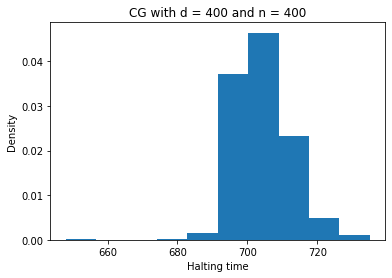
\includegraphics[width=0.38\linewidth]{part-3-images/illconditioned.png}
%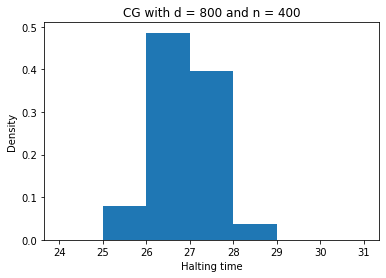
\includegraphics[width=0.38\linewidth]{part-3-images/wellconditioned.png}
\begin{overpic}[width=0.38\linewidth]{part-3-images/between.png}
\put(65,50){\only<4>{\textcolor{red}{\rotatebox{0}{\boxed{``in~ between"}}}}}
\end{overpic}
\end{center}
\end{frame}


\begin{frame}{Qualitative comparison with SGD}
\begin{columns}
\begin{column}{0.4\textwidth}

  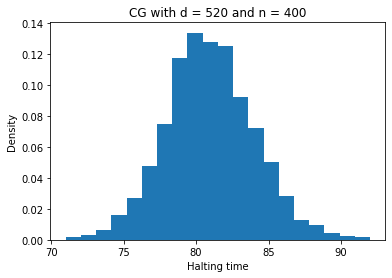
\includegraphics[width=\linewidth]{part-3-images/between.png}\\
  
  \shadowimage[width=\linewidth]{part-1-images/sagun_fig3a.png}
  \end{column}
  \begin{column}{0.48\textwidth}
  \only<1>{While the mechanisms behind these behaviors are surely different, we see a non-trivial histogram in each setting. 
  \vspace{.1in}
  
  For CG on Wishart matrices, it can be shown that
  \begin{align*}
      \|\boldsymbol r_{k}\| = \|\cc - \AA^T \AA \boldsymbol x_k\| \overset{\mathrm{(dist)}}{=} \prod_{j=0}^{k-1} \frac{\chi_{n - j -1 }}{\chi_{d - j}},
  \end{align*}
  for independent chi-distributed random variables.}
  
  \only<2>{So, if we set \begin{align*}
      E_k(\mathrm{Wishart};\mathrm{CG}) =  \|\boldsymbol r_{k}\|
  \end{align*} we can analyze the halting time to see that
  \begin{align*}
      T_{\mathrm{CG}}(\mathrm{Wishart},\epsilon) &\approx \frac{2}{c} n^{1 - \alpha} \log \epsilon^{-1}\\
      &+ O(n^{3/2-2\alpha}) \mathcal N(0,1),
  \end{align*}
  for $1/2 < \alpha < 1$.}
  \end{column}
  \end{columns}
\end{frame}



\begin{frame}{To the well-conditioned regime!}
\begin{center}
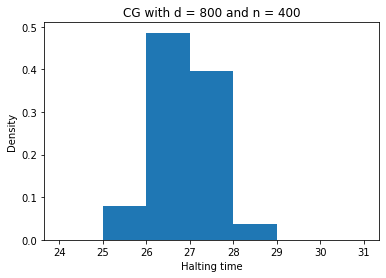
\includegraphics[width=.5\linewidth]{part-3-images/wellconditioned.png}
\end{center}

\only<1>{It turns out that the errors $E_k(P_N;\mathcal A)$ for iterative methods for a linear system involving $\AA^T\AA$ are often analyzable in the well-conditioned, ill-conditioned and ``in between" regimes.  But the analysis of the halting time can be much more involved because the halting time $T_{\mathcal A}(P_n,\epsilon)$ can tend to infinity with $n$!}
\only<2>{\begin{center}So, we, for the time being, let $d = \lfloor n r \rfloor$ for $r > 1$.\end{center}}

\end{frame}


\begin{frame}{Polynomials!}

\hspace{2in}\boxed{\text{The Gradient Descent Algorithm \label{a:gd}}}
\begin{enumerate}
    \item $\boldsymbol x_0$ is the initial vector.
    \item For $k = 1,2,\ldots$
    \begin{enumerate}
        \item Select step size $\gamma_k$
        \item Compute $\xx_k = \xx_{k-1} - \gamma_k \nabla \mathcal L(\xx_{k-1})$
    \end{enumerate}
\end{enumerate}

\pause

Recall that the gradient of the regression functional is
\begin{align*}
    \nabla \mathcal L(\xx)  = \WW \xx - \cc, \quad \WW = \frac{\AA^T \AA}{d}.
\end{align*}
%and for some collection of step sizes $\gamma_k$, the GD iteration is given by:

\pause


A direction calculation reveals that
\begin{align*}
    \xx_k = Q_k(\WW) \cc,
\end{align*}
for a polynomial $Q_k$ of degree $k-1$ with coefficients that depend on $\gamma_j$, $j =1,2,\ldots,k$. 

\end{frame}



\begin{frame}{More polynomials!}
% It follows that
% \begin{align*}
%     \xx_{k} \in \mathrm{span}\{\cc, \WW \cc, \WW^2 \cc, \ldots,\WW^{k-1} \cc\}.
% \end{align*}
% As we will see, norms of such vectors are often analyzable with RMT.

% \pause
% \vspace{.1in}

For simplicity, suppose that $\WW$ is full rank.  Then if $\xx$ is the true minimizer, a crucial calculation is that
\begin{align*}
    \xx - \xx_k = \WW^{-1} \cc - Q_k(\WW)\cc = \WW^{-1} \underbrace{(\II_n - \WW Q_k(\WW))}_{R_k(\WW)} \cc.
\end{align*}
Note that $R_k$ is a polynomial of degree $k$ satisfying $R_k(0) = 1$.

\vspace{.1in}

Then
\begin{align*}
    \nabla \mathcal L(\xx_k) &= \WW \xx_k - \WW \xx = R_k(\WW) \cc,\\
    \|R_k(\WW) \cc\|^2 &= \cc^T R_k(\WW)^2 \cc.
\end{align*}

\end{frame}

\begin{frame}{Example: GD}
For GD follows that the difference $\xx_k - \xx$ satisfies
\begin{align*}
\xx_k - \xx = \xx_{k-1} - \xx - \gamma_k (W \xx_{k-1} - W \xx) = (\II_n - \gamma_k W) (\xx_{k-1} - \xx).
\end{align*}
And so,
\begin{align*}
    R_k(x) = \prod_{j=1}^k (1 - \gamma_j x).
\end{align*}
\pause

For CG the polynomial $R_k$ is best characterized using the theory of orthogonal polynomials.


\end{frame}


\begin{frame}{Enter RMT}
\begin{align*}
    \|R_k(\WW) \cc\|^2 &= \cc^T R_k(\WW)^2 \cc
\end{align*}

The error analysis of GD (and, as it turns out, CG) is reduced to:
\begin{enumerate}
    \item The determination/characterization of the polynomial $R_k$.
    \item The estimation of $\cc^T R_k(\WW)^2 \cc$.
\end{enumerate}
\end{frame}



\begin{frame}{Enter RMT}

For many methods of interest (CG and GD included), the coefficients of $R_k$ depend continuously on the eigenvalues and eigenvectors of $\WW$ in a sufficiently strong sense that
\begin{align*}
    R_k(x) \Prto{n} \mathcal R_k(x)   \longleftarrow \text{\textcolor{red}{deterministic}}.
\end{align*}

Then, one can conclude
\begin{align*}
    \cc^T R_k(\WW)^2 \cc \Prto{n} \int_{\mathbb R} \mathcal R_k(x)^2 \mu_{\mathrm{SCM}}(\dif x).
\end{align*}

This provides a deterministic limit for the (random) errors that are encountered throughout the algorithm.

Note:  This is true only if $\cc$ is independent of $\WW$ and in the regression problem it is not. 

\end{frame}

\begin{frame}{Building back to true regression}
For the regression problem, we have
\begin{align*}
    \cc = \frac{1}{n} \left[\AA^T\AA \aa + \AA^T \eeta \right].
\end{align*}
Then
\begin{align*}
    \| \mathcal L(\xx_k) \|^2 = \aa^T \WW^2 R_k(\WW)^2 \aa^T + \frac{1}{n^2} \eeta^T \AA R_k(\WW)^2 \AA^T \eeta + \underbrace{\frac{2}{n} \aa^T \WW R_k(\WW)^2 \AA^T \eeta}_{\only<2->{\approx 0 ~~ \text{if} ~~ \aa, \eeta \text{ indep.}}}\\
    \uncover<3->{\Prto{n} \underbrace{R \int_{\mathbb R}x^2 \mathcal R_k(x)^2 \mu_{\mathrm{SCM}}(\dif x) + \tilde R \int_{\mathbb R} x \mathcal R_k(x)^2 \mu_{\mathrm{SCM}}(\dif x)}_{\mathfrak e_k^2}.}
\end{align*}


\uncover<4->{Important features:
\begin{itemize}
    \item This demonstrates that the entire spectrum of $\WW$ contributes via $\mu_{\mathrm{SCM}}$
    \item Nearly all probabilistic analyses of algorithms give inequalities whereas this gives true leading-order behavior.
\end{itemize}
}
\end{frame}

\begin{frame}{Step-size selection}
    \begin{align*}
        \| \mathcal L(\xx_k) \|^2 \Prto{n} R \int_{\mathbb R}x^2 \mathcal R_k(x)^2 \mu_{\mathrm{SCM}}(\dif x) + \tilde R \int_{\mathbb R} x \mathcal R_k(x)^2 \mu_{\mathrm{SCM}}(\dif x)
    \end{align*}
    
    If one has a good guess as to what the limiting distribution $\mu_{\mathrm{SCM}}$ is then the $\gamma_k$'s in GD can be chosen based on this limit --- to minimize this expression, see \cite{pedregosa2020acceleration}.
    
    \pause
    
    Furthermore, by preconditioning one can make such a guess valid, see \cite{lacotte2020optimal}.
\end{frame}

\begin{frame}{Deterministic halting}
Provided that $\mathfrak e_k \To{k} 0$, one finds that
\begin{align*}
    \lim_{n \to \infty} \mathbb P \left( T_{\mathcal A}(P_n;\epsilon) = \min \{ k : \mathfrak e_k < \epsilon \} \right) = 1,
\end{align*}
for most choices of $\epsilon$.\\
\vspace{.1in}

This turns out to be true for all $d \geq n$, $n \to \infty,$ for the regression problem with CG or GD.
\end{frame}

\begin{frame}{Deterministic halting for CG with $r = 2$, $\epsilon = 10^{-4}$}
\begin{center}
\pause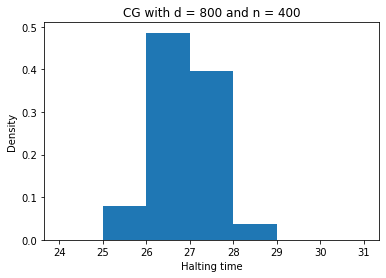
\includegraphics[width=0.38\linewidth]{part-3-images/wellconditioned.png}\pause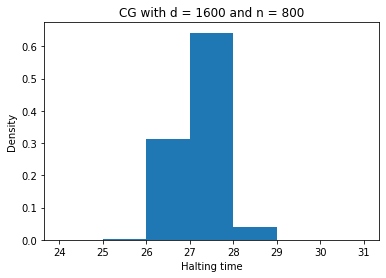
\includegraphics[width=0.38\linewidth]{part-3-images/800.png}\\
\pause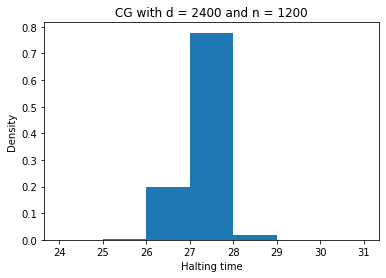
\includegraphics[width=0.38\linewidth]{part-3-images/1200.png}\pause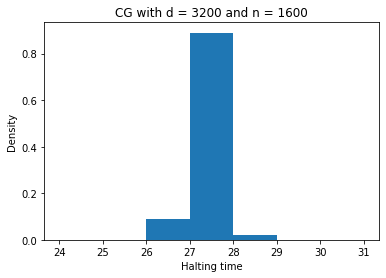
\includegraphics[width=0.38\linewidth]{part-3-images/1600.png}
\end{center}
\end{frame}

% \begin{frame}{Catalog of results}
%   Signal processing -- Vershynin, Strohmer on randomize Kaczmarz.  Matrix completion.
  
%   Results for SGD. randomize Kaczmarz
% \end{frame}




\begin{frame}{Outlook}
    RMT provides non-trivial tractable models to analyze the statistics of optimization algorithms.\\
    
    \vspace{.05in}
    
    Other algorithms are analyzable:
    \begin{itemize}
        \item MINRES algorithm
        \item Polyak algorithm
        \item Nesterov accelerated algorithm
        \item SGD for regression
        \item $\ldots$
    \end{itemize}
    See the preprints: \cite{paquette2020universality,Paquette2021,Ding2021,Paquette2020a}

    \end{frame}
    
    \begin{frame}{Outlook}

    Other ensembles are analyzable using the following results from RMT:
    \begin{itemize}
        \item Spiked random matrices (see \cite{Baik2005,Bloemendal2013,Ding2019}, and many more)
        \item Nonlinear models (see Part 4)
        \item Random graphs (see \cite{Erdos2013a}, for example)
        \item Invariant ensembles (see \cite{Bourgade2014,DeiftOrthogonalPolynomials} and many more)
    \end{itemize}

    \end{frame}
    
    \begin{frame}{Open questions}
    Many open questions remain:
    \begin{itemize}
        \item \pause To what extent can one move these ideas beyond regression?  To a two-layer network?  Rank-one matrix completion problem?
        \item \pause What is a good probability distribution to study? Wishart is clearly the place to start but what is relevant in practice?
    \end{itemize}
\end{frame}

\begin{frame}{A CG demo}
\begin{center}
See Colab for a CG demo\\
 \url{https://colab.research.google.com/drive/1UZRSK665b8sqq0NQFwMCwrVabPlB-7nK?usp=sharing}
\end{center}
\end{frame}


\begin{frame}[allowframebreaks]{References}
%\bibliographystyle{notplainnat}
 %\bibliography{references}
\bibliographystyle{plainnat}
  {\scriptsize\bibliography{references}}

\end{frame}

\end{document}


































































\begin{frame}{Table of contents}
  \setbeamertemplate{section in toc}[sections numbered]
  \tableofcontents%[hideallsubsections]
\end{frame}

\section[Intro]{Introduction}

\begin{frame}[fragile]{Metropolis}

  The \themename theme is a Beamer theme with minimal visual noise
  inspired by the \href{https://github.com/hsrmbeamertheme/hsrmbeamertheme}{\textsc{hsrm} Beamer
  Theme} by Benjamin Weiss.

  Enable the theme by loading

  \begin{verbatim}    \documentclass{beamer}
    \usetheme{metropolis}\end{verbatim}

  Note, that you have to have Mozilla's \emph{Fira Sans} font and XeTeX
  installed to enjoy this wonderful typography.
\end{frame}
\begin{frame}[fragile]{Sections}
  Sections group slides of the same topic

  \begin{verbatim}    \section{Elements}\end{verbatim}

  for which \themename provides a nice progress indicator \ldots
  
\end{frame}

\section{Titleformats}

\begin{frame}{Metropolis titleformats}
	\themename supports 4 different titleformats:
	\begin{itemize}
		\item Regular
		\item \textsc{Smallcaps}
		\item \textsc{allsmallcaps}
		\item ALLCAPS
	\end{itemize}
	They can either be set at once for every title type or individually.
\end{frame}

\subsection{Tricks}

{
    \metroset{titleformat frame=smallcaps}
\begin{frame}{Small caps}
	This frame uses the \texttt{smallcaps} titleformat.

	\begin{alertblock}{Potential Problems}
		Be aware, that not every font supports small caps. If for example you typeset your presentation with pdfTeX and the Computer Modern Sans Serif font, every text in smallcaps will be typeset with the Computer Modern Serif font instead.
	\end{alertblock}
\end{frame}
}

{
\metroset{titleformat frame=allsmallcaps}
\begin{frame}{All small caps}
	This frame uses the \texttt{allsmallcaps} titleformat.

	\begin{alertblock}{Potential problems}
		As this titleformat also uses smallcaps you face the same problems as with the \texttt{smallcaps} titleformat. Additionally this format can cause some other problems. Please refer to the documentation if you consider using it.

		As a rule of thumb: Just use it for plaintext-only titles.
	\end{alertblock}
\end{frame}
}

{
\metroset{titleformat frame=allcaps}
\begin{frame}{All caps}
	This frame uses the \texttt{allcaps} titleformat.

	\begin{alertblock}{Potential Problems}
		This titleformat is not as problematic as the \texttt{allsmallcaps} format, but basically suffers from the same deficiencies. So please have a look at the documentation if you want to use it.
	\end{alertblock}
\end{frame}
}

\section{Elements}

\begin{frame}[fragile]{Typography}
      \begin{verbatim}The theme provides sensible defaults to
\emph{emphasize} text, \alert{accent} parts
or show \textbf{bold} results.\end{verbatim}

  \begin{center}becomes\end{center}

  The theme provides sensible defaults to \emph{emphasize} text,
  \alert{accent} parts or show \textbf{bold} results.
\end{frame}

\begin{frame}{Font feature test}
  \begin{itemize}
    \item Regular
    \item \textit{Italic}
    \item \textsc{SmallCaps}
    \item \textbf{Bold}
    \item \textbf{\textit{Bold Italic}}
    \item \textbf{\textsc{Bold SmallCaps}}
    \item \texttt{Monospace}
    \item \texttt{\textit{Monospace Italic}}
    \item \texttt{\textbf{Monospace Bold}}
    \item \texttt{\textbf{\textit{Monospace Bold Italic}}}
  \end{itemize}
\end{frame}

\begin{frame}{Lists}
  \begin{columns}[T,onlytextwidth]
    \column{0.33\textwidth}
      Items
      \begin{itemize}
        \item Milk \item Eggs \item Potatos
      \end{itemize}

    \column{0.33\textwidth}
      Enumerations
      \begin{enumerate}
        \item First, \item Second and \item Last.
      \end{enumerate}

    \column{0.33\textwidth}
      Descriptions
      \begin{description}
        \item[PowerPoint] Meeh. \item[Beamer] Yeeeha.
      \end{description}
  \end{columns}
\end{frame}
\begin{frame}{Animation}
  \begin{itemize}[<+- | alert@+>]
    \item \alert<4>{This is\only<4>{ really} important}
    \item Now this
    \item And now this
  \end{itemize}
\end{frame}
\begin{frame}{Figures}
  \begin{figure}
    \newcounter{density}
    \setcounter{density}{20}
    \begin{tikzpicture}
      \def\couleur{alerted text.fg}
      \path[coordinate] (0,0)  coordinate(A)
                  ++( 90:5cm) coordinate(B)
                  ++(0:5cm) coordinate(C)
                  ++(-90:5cm) coordinate(D);
      \draw[fill=\couleur!\thedensity] (A) -- (B) -- (C) --(D) -- cycle;
      \foreach \x in {1,...,40}{%
          \pgfmathsetcounter{density}{\thedensity+20}
          \setcounter{density}{\thedensity}
          \path[coordinate] coordinate(X) at (A){};
          \path[coordinate] (A) -- (B) coordinate[pos=.10](A)
                              -- (C) coordinate[pos=.10](B)
                              -- (D) coordinate[pos=.10](C)
                              -- (X) coordinate[pos=.10](D);
          \draw[fill=\couleur!\thedensity] (A)--(B)--(C)-- (D) -- cycle;
      }
    \end{tikzpicture}
    \caption{Rotated square from
    \href{http://www.texample.net/tikz/examples/rotated-polygons/}{texample.net}.}
  \end{figure}
\end{frame}
\begin{frame}{Tables}
  \begin{table}
    \caption{Largest cities in the world (source: Wikipedia)}
    \begin{tabular}{lr}
      \toprule
      City & Population\\
      \midrule
      Mexico City & 20,116,842\\
      Shanghai & 19,210,000\\
      Peking & 15,796,450\\
      Istanbul & 14,160,467\\
      \bottomrule
    \end{tabular}
  \end{table}
\end{frame}
\begin{frame}{Blocks}
  Three different block environments are pre-defined and may be styled with an
  optional background color.

  \begin{columns}[T,onlytextwidth]
    \column{0.5\textwidth}
      \begin{block}{Default}
        Block content.
      \end{block}

      \begin{alertblock}{Alert}
        Block content.
      \end{alertblock}

      \begin{exampleblock}{Example}
        Block content.
      \end{exampleblock}

    \column{0.5\textwidth}

      \metroset{block=fill}

      \begin{block}{Default}
        Block content.
      \end{block}

      \begin{alertblock}{Alert}
        Block content.
      \end{alertblock}

      \begin{exampleblock}{Example}
        Block content.
      \end{exampleblock}

  \end{columns}
\end{frame}
\begin{frame}{Math}
  \begin{equation*}
    e = \lim_{n\to \infty} \left(1 + \frac{1}{n}\right)^n
  \end{equation*}
\end{frame}
\begin{frame}{Line plots}
  \begin{figure}
    \begin{tikzpicture}
      \begin{axis}[
        mlineplot,
        width=0.9\textwidth,
        height=6cm,
      ]

        \addplot {sin(deg(x))};
        \addplot+[samples=100] {sin(deg(2*x))};

      \end{axis}
    \end{tikzpicture}
  \end{figure}
\end{frame}
\begin{frame}{Bar charts}
  \begin{figure}
    \begin{tikzpicture}
      \begin{axis}[
        mbarplot,
        xlabel={Foo},
        ylabel={Bar},
        width=0.9\textwidth,
        height=6cm,
      ]

      \addplot plot coordinates {(1, 20) (2, 25) (3, 22.4) (4, 12.4)};
      \addplot plot coordinates {(1, 18) (2, 24) (3, 23.5) (4, 13.2)};
      \addplot plot coordinates {(1, 10) (2, 19) (3, 25) (4, 15.2)};

      \legend{lorem, ipsum, dolor}

      \end{axis}
    \end{tikzpicture}
  \end{figure}
\end{frame}
\begin{frame}{Quotes}
  \begin{quote}
    Veni, Vidi, Vici
  \end{quote}
\end{frame}

{%
\setbeamertemplate{frame footer}{My custom footer}
\begin{frame}[fragile]{Frame footer}
    \themename defines a custom beamer template to add a text to the footer. It can be set via
    \begin{verbatim}\setbeamertemplate{frame footer}{My custom footer}\end{verbatim}
\end{frame}
}

\begin{frame}{References}
  Some references to showcase [allowframebreaks] \cite{knuth92,ConcreteMath,Simpson,Er01,greenwade93}
\end{frame}

\section{Conclusion}

\begin{frame}{Summary}

  Get the source of this theme and the demo presentation from

  \begin{center}\url{github.com/matze/mtheme}\end{center}

  The theme \emph{itself} is licensed under a
  \href{http://creativecommons.org/licenses/by-sa/4.0/}{Creative Commons
  Attribution-ShareAlike 4.0 International License}.

  \begin{center}\ccbysa\end{center}

\end{frame}

{\setbeamercolor{palette primary}{fg=black, bg=yellow}
\begin{frame}[standout]
  Questions?
\end{frame}
}

\appendix

\begin{frame}[fragile]{Backup slides}
  Sometimes, it is useful to add slides at the end of your presentation to
  refer to during audience questions.

  The best way to do this is to include the \verb|appendixnumberbeamer|
  package in your preamble and call \verb|\appendix| before your backup slides.

  \themename will automatically turn off slide numbering and progress bars for
  slides in the appendix.
\end{frame}

\begin{frame}[allowframebreaks]{References}

  %\bibliography{demo}
  \bibliographystyle{abbrv}

\end{frame}

\end{document}
